\documentclass{article}
\usepackage{tikz}
\usepackage{graphicx}
\usepackage{amsmath}

\begin{document}
\usetikzlibrary{arrows.meta, positioning}

% Remove page numbers
\pagestyle{empty}

% Schematic Diagram
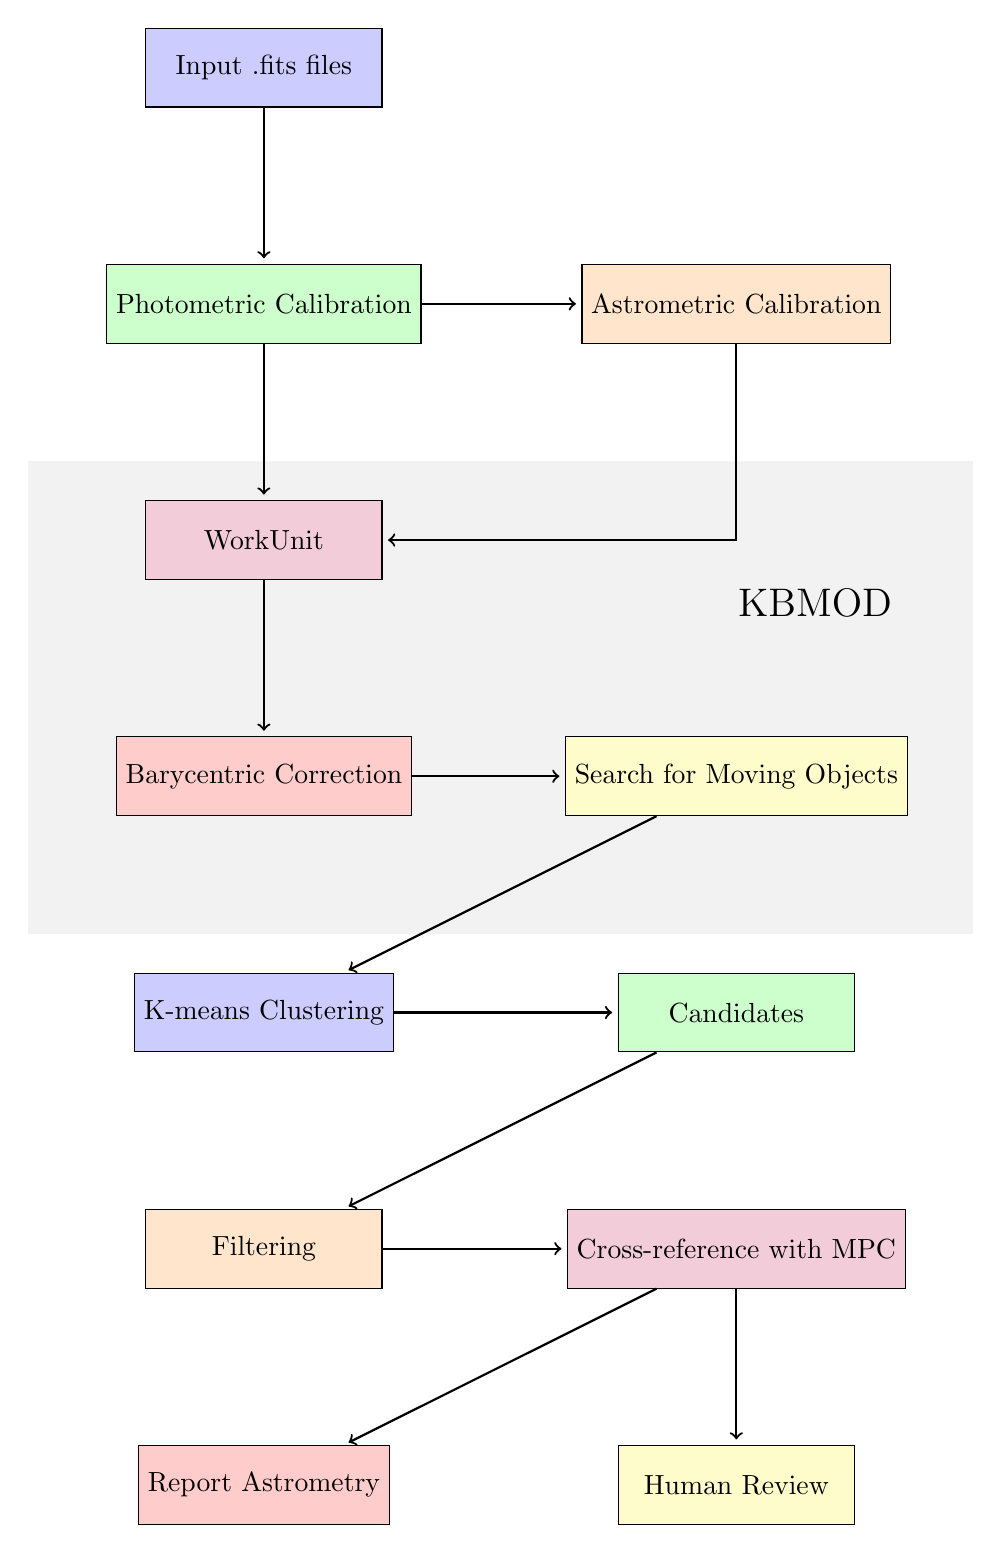
\begin{tikzpicture}[node distance=2cm]

% Add rectangle to behind the workunit, barycentric correction, and search for moving objects
\node (background) [rectangle, draw=none, fill=gray!10, minimum width=12cm, minimum height=6cm, yshift=-8cm, xshift=3cm, label={[yshift=1.2cm, xshift=4cm, font=\Large]center:KBMOD}] {};

% Input .fits files
\node (input) [rectangle, draw, fill=blue!20, minimum width=3cm, minimum height=1cm] {Input .fits files};

% Calibration
\node (photometric_calibration) [rectangle, draw, fill=green!20, minimum width=3cm, minimum height=1cm, below of=input, yshift=-1cm] {Photometric Calibration};

% Source Extraction
\node (astrometric_calibration) [rectangle, draw, fill=orange!20, minimum width=3cm, minimum height=1cm, right of=photometric_calibration, xshift=4cm] {Astrometric Calibration};

% Combine .fits files into KBMOD WorkUnit
\node (combine) [rectangle, draw, fill=purple!20, minimum width=3cm, minimum height=1cm, below of=photometric_calibration, yshift=-1cm] {WorkUnit};

% Barycentric Correction
\node (barycentric_correction) [rectangle, draw, fill=red!20, minimum width=3cm, minimum height=1cm, below of=combine, yshift=-1cm] {Barycentric Correction};

% Search for Moving Objects right of Barycentric Correction
\node (search) [rectangle, draw, fill=yellow!20, minimum width=3cm, minimum height=1cm, right of=barycentric_correction, xshift=4cm] {Search for Moving Objects};


% K-means Clustering
\node (clustering) [rectangle, draw, fill=blue!20, minimum width=3cm, minimum height=1cm, below of=barycentric_correction, yshift=-1cm] {K-means Clustering};

% K-means Clustering below Search for Moving Objects
\node (candidates) [rectangle, draw, fill=green!20, minimum width=3cm, minimum height=1cm, below of=search, yshift=-1cm] {Candidates};

% Candidate Validation
\node (filtering) [rectangle, draw, fill=orange!20, minimum width=3cm, minimum height=1cm, below of=clustering, yshift=-1cm] {Filtering};

% Cross-reference with MPC
\node (mpc) [rectangle, draw, fill=purple!20, minimum width=3cm, minimum height=1cm, below of=candidates, yshift=-1cm] {Cross-reference with MPC};

% Output
\node (output) [rectangle, draw, fill=red!20, minimum width=3cm, minimum height=1cm, below of=filtering, yshift=-1cm] {Report Astrometry};

% Human Review
\node (human_review) [rectangle, draw, fill=yellow!20, minimum width=3cm, minimum height=1cm, below of=mpc, yshift=-1cm] {Human Review};

% Arrows
\draw[->, thick, shorten >= 2pt] (input) -- (photometric_calibration);
\draw[->, thick, shorten >= 2pt] (photometric_calibration) -- (combine);
\draw[->, thick, shorten >= 2pt] (photometric_calibration) -- (astrometric_calibration);
\draw[->, thick, shorten >= 2pt] (astrometric_calibration) |- (combine);
\draw[->, thick, shorten >= 2pt] (combine) -- (barycentric_correction);
\draw[->, thick, shorten >= 2pt] (barycentric_correction) -- (search);
\draw[->, thick, shorten >= 2pt] (search) -- (clustering);
\draw[->, thick, shorten >= 2pt] (clustering) -- (candidates);
\draw[->, thick, shorten >= 2pt] (candidates) -- (filtering);
\draw[->, thick, shorten >= 2pt] (filtering) -- (mpc);
\draw[->, thick, shorten >= 2pt] (mpc) -- (human_review);
\draw[->, thick, shorten >= 2pt] (mpc) -- (output);

\end{tikzpicture}


% end document
\end{document}